% ---------------------------------------------------------------------------
% ---------------------------------------------------------------------------
% Modelo LaTex para preparação do documento final de Monografia TCC
% O modelo está em conformidade com ABNT NBR
% Faculdade do Piaui
% ---------------------------------------------------------------------------
% ---------------------------------------------------------------------------

\documentclass[
	% -- opções da classe memoir --
	12pt,					% tamanho da fonte
	book,				% capítulos começam em pág ímpar (insere página vazia caso preciso)
	oneside,					% para impressão em verso e anverso. Oposto a oneside
	a4paper,					% tamanho do papel. 
	% -- opções da classe abntex2 --
	%chapter=TITLE,			% títulos de capítulos convertidos em letras maiúsculas
	%section=TITLE,			% títulos de seções convertidos em letras maiúsculas
	%subsection=TITLE,		% títulos de subseções convertidos em letras maiúsculas
	%subsubsection=TITLE,	% títulos de subsubseções convertidos em letras maiúsculas
	% -- opções do pacote babel --
	english,					% idioma adicional para hifenização
	%french,					% idioma adicional para hifenização
	%spanish,				% idioma adicional para hifenização
	brazil					% o último idioma é o principal do documento
	]{abntex2}

% ---------------------
% Pacotes OBRIGATÓRIOS
% ---------------------
\usepackage{lmodern}				% Usa a fonte Latin Modern			
\usepackage[T1]{fontenc}			% Selecao de codigos de fonte.
\usepackage[utf8]{inputenc}		% Codificacao do documento (conversão automática dos acentos)
\usepackage{lastpage}			% Usado pela Ficha catalográfica
\usepackage{indentfirst}			% Indenta o primeiro parágrafo de cada seção.
\usepackage{color}				% Controle das cores
\usepackage{graphicx}	% Inclusão de gráficos
\graphicspath{{figs/}}
\usepackage{epsfig,subfig}		% Inclusão de figuras
\usepackage{microtype} 			% Melhorias de justificação
\usepackage[table,xcdraw]{xcolor}
% ---------------------	
% ---------------------
% Pacotes ADICIONAIS
% ---------------------
\usepackage{pdfpages}
\usepackage{lipsum}						% Geração de dummy text
\usepackage{amsmath,amssymb,mathrsfs}	% Comandos matemáticos avançados 
\usepackage{setspace}  					% Para permitir espaçamento simples, 1 1/2 e duplo
\usepackage{verbatim}					% Para poder usar o ambiente "comment"
\usepackage{tabularx} 					% Para poder ter tabelas com colunas de largura auto-ajustável
\usepackage{afterpage} 					% Para executar um comando depois do fim da página corrente
\usepackage{url} 						% Para formatar URLs (endereços da Web)
%pacote arduino
\usepackage{listings} 
\usepackage{float}
 %%%%%%%%%%%%%%%%%%%%%%%%%%%%%%%%%%%%%%%%%%%%%%%%%%%%%%%%%%%%%%%%%%%%%%%%%%%%%%%% 
%%% ~ Arduino Language - Arduino IDE Colors ~                                  %%%
%%%                                                                            %%%
%%% Kyle Rocha-Brownell | 10/2/2017 | No Licence                               %%%
%%% -------------------------------------------------------------------------- %%%
%%%                                                                            %%%
%%% Place this file in your working directory (next to the latex file you're   %%%
%%% working on).  To add it to your project, place:                            %%%
%%%     %%%%%%%%%%%%%%%%%%%%%%%%%%%%%%%%%%%%%%%%%%%%%%%%%%%%%%%%%%%%%%%%%%%%%%%%%%%%%%%% 
%%% ~ Arduino Language - Arduino IDE Colors ~                                  %%%
%%%                                                                            %%%
%%% Kyle Rocha-Brownell | 10/2/2017 | No Licence                               %%%
%%% -------------------------------------------------------------------------- %%%
%%%                                                                            %%%
%%% Place this file in your working directory (next to the latex file you're   %%%
%%% working on).  To add it to your project, place:                            %%%
%%%     %%%%%%%%%%%%%%%%%%%%%%%%%%%%%%%%%%%%%%%%%%%%%%%%%%%%%%%%%%%%%%%%%%%%%%%%%%%%%%%% 
%%% ~ Arduino Language - Arduino IDE Colors ~                                  %%%
%%%                                                                            %%%
%%% Kyle Rocha-Brownell | 10/2/2017 | No Licence                               %%%
%%% -------------------------------------------------------------------------- %%%
%%%                                                                            %%%
%%% Place this file in your working directory (next to the latex file you're   %%%
%%% working on).  To add it to your project, place:                            %%%
%%%    \input{arduinoLanguage.tex}                                             %%%
%%% somewhere before \begin{document} in your latex file.                      %%%
%%%                                                                            %%%
%%% In your document, place your arduino code between:                         %%%
%%%   \begin{lstlisting}[language=Arduino]                                     %%%
%%% and:                                                                       %%%
%%%   \end{lstlisting}                                                         %%%
%%%                                                                            %%%
%%% Or create your own style to add non-built-in functions and variables.      %%%
%%%                                                                            %%%
 %%%%%%%%%%%%%%%%%%%%%%%%%%%%%%%%%%%%%%%%%%%%%%%%%%%%%%%%%%%%%%%%%%%%%%%%%%%%%%%% 

\usepackage{color}
\usepackage{listings}    
\usepackage{courier}

%%% Define Custom IDE Colors %%%
\definecolor{arduinoGreen}    {rgb} {0.17, 0.43, 0.01}
\definecolor{arduinoGrey}     {rgb} {0.47, 0.47, 0.33}
\definecolor{arduinoOrange}   {rgb} {0.8 , 0.4 , 0   }
\definecolor{arduinoBlue}     {rgb} {0.01, 0.61, 0.98}
\definecolor{arduinoDarkBlue} {rgb} {0.0 , 0.2 , 0.5 }
\definecolor{MyLightGray}{RGB}{235, 235,235}
%%% Define Arduino Language %%%
\lstdefinelanguage{Arduino}{
  language=C++, % begin with default C++ settings 
%
%
  %%% Keyword Color Group 1 %%%  (called KEYWORD3 by arduino)
  keywordstyle=\color{arduinoGreen},
  backgroundcolor=\color{MyLightGray},   
  deletekeywords={  % remove all arduino keywords that might be in c++
                break, case, override, final, continue, default, do, else, for, 
                if, return, goto, switch, throw, try, while, setup, loop, export, 
                not, or, and, xor, include, define, elif, else, error, if, ifdef, 
                ifndef, pragma, warning,
                HIGH, LOW, INPUT, INPUT_PULLUP, OUTPUT, DEC, BIN, HEX, OCT, PI, 
                HALF_PI, TWO_PI, LSBFIRST, MSBFIRST, CHANGE, FALLING, RISING, 
                DEFAULT, EXTERNAL, INTERNAL, INTERNAL1V1, INTERNAL2V56, LED_BUILTIN, 
                LED_BUILTIN_RX, LED_BUILTIN_TX, DIGITAL_MESSAGE, FIRMATA_STRING, 
                ANALOG_MESSAGE, REPORT_DIGITAL, REPORT_ANALOG, SET_PIN_MODE, 
                SYSTEM_RESET, SYSEX_START, auto, int8_t, int16_t, int32_t, int64_t, 
                uint8_t, uint16_t, uint32_t, uint64_t, char16_t, char32_t, operator, 
                enum, delete, bool, boolean, byte, char, const, false, float, double, 
                null, NULL, int, long, new, private, protected, public, short, 
                signed, static, volatile, String, void, true, unsigned, word, array, 
                sizeof, dynamic_cast, typedef, const_cast, struct, static_cast, union, 
                friend, extern, class, reinterpret_cast, register, explicit, inline, 
                _Bool, complex, _Complex, _Imaginary, atomic_bool, atomic_char, 
                atomic_schar, atomic_uchar, atomic_short, atomic_ushort, atomic_int, 
                atomic_uint, atomic_long, atomic_ulong, atomic_llong, atomic_ullong, 
                virtual, PROGMEM,
                Serial, Serial1, Serial2, Serial3, SerialUSB, Keyboard, Mouse,
                abs, acos, asin, atan, atan2, ceil, constrain, cos, degrees, exp, 
                floor, log, map, max, min, radians, random, randomSeed, round, sin, 
                sq, sqrt, tan, pow, bitRead, bitWrite, bitSet, bitClear, bit, 
                highByte, lowByte, analogReference, analogRead, 
                analogReadResolution, analogWrite, analogWriteResolution, 
                attachInterrupt, detachInterrupt, digitalPinToInterrupt, delay, 
                delayMicroseconds, digitalWrite, digitalRead, interrupts, millis, 
                micros, noInterrupts, noTone, pinMode, pulseIn, pulseInLong, shiftIn, 
                shiftOut, tone, yield, Stream, begin, end, peek, read, print, 
                println, available, availableForWrite, flush, setTimeout, find, 
                findUntil, parseInt, parseFloat, readBytes, readBytesUntil, readString, 
                readStringUntil, trim, toUpperCase, toLowerCase, charAt, compareTo, 
                concat, endsWith, startsWith, equals, equalsIgnoreCase, getBytes, 
                indexOf, lastIndexOf, length, replace, setCharAt, substring, 
                toCharArray, toInt, press, release, releaseAll, accept, click, move, 
                isPressed, isAlphaNumeric, isAlpha, isAscii, isWhitespace, isControl, 
                isDigit, isGraph, isLowerCase, isPrintable, isPunct, isSpace, 
                isUpperCase, isHexadecimalDigit, 
                }, 
  morekeywords={   % add arduino structures to group 1
                break, case, override, final, continue, default, do, else, for, 
                if, return, goto, switch, throw, try, while, setup, loop, export, 
                not, or, and, xor, include, define, elif, else, error, if, ifdef, 
                ifndef, pragma, warning,
                }, 
% 
%
  %%% Keyword Color Group 2 %%%  (called LITERAL1 by arduino)
  keywordstyle=[2]\color{arduinoBlue},   
  keywords=[2]{   % add variables and dataTypes as 2nd group  
                HIGH, LOW, INPUT, INPUT_PULLUP, OUTPUT, DEC, BIN, HEX, OCT, PI, 
                HALF_PI, TWO_PI, LSBFIRST, MSBFIRST, CHANGE, FALLING, RISING, 
                DEFAULT, EXTERNAL, INTERNAL, INTERNAL1V1, INTERNAL2V56, LED_BUILTIN, 
                LED_BUILTIN_RX, LED_BUILTIN_TX, DIGITAL_MESSAGE, FIRMATA_STRING, 
                ANALOG_MESSAGE, REPORT_DIGITAL, REPORT_ANALOG, SET_PIN_MODE, 
                SYSTEM_RESET, SYSEX_START, auto, int8_t, int16_t, int32_t, int64_t, 
                uint8_t, uint16_t, uint32_t, uint64_t, char16_t, char32_t, operator, 
                enum, delete, bool, boolean, byte, char, const, false, float, double, 
                null, NULL, int, long, new, private, protected, public, short, 
                signed, static, volatile, String, void, true, unsigned, word, array, 
                sizeof, dynamic_cast, typedef, const_cast, struct, static_cast, union, 
                friend, extern, class, reinterpret_cast, register, explicit, inline, 
                _Bool, complex, _Complex, _Imaginary, atomic_bool, atomic_char, 
                atomic_schar, atomic_uchar, atomic_short, atomic_ushort, atomic_int, 
                atomic_uint, atomic_long, atomic_ulong, atomic_llong, atomic_ullong, 
                virtual, PROGMEM,
                },  
% 
%
  %%% Keyword Color Group 3 %%%  (called KEYWORD1 by arduino)
  keywordstyle=[3]\bfseries\color{arduinoOrange},
  keywords=[3]{  % add built-in functions as a 3rd group
                Serial, Serial1, Serial2, Serial3, SerialUSB, Keyboard, Mouse,
                },      
%
%
  %%% Keyword Color Group 4 %%%  (called KEYWORD2 by arduino)
  keywordstyle=[4]\color{arduinoOrange},
  keywords=[4]{  % add more built-in functions as a 4th group
                abs, acos, asin, atan, atan2, ceil, constrain, cos, degrees, exp, 
                floor, log, map, max, min, radians, random, randomSeed, round, sin, 
                sq, sqrt, tan, pow, bitRead, bitWrite, bitSet, bitClear, bit, 
                highByte, lowByte, analogReference, analogRead, 
                analogReadResolution, analogWrite, analogWriteResolution, 
                attachInterrupt, detachInterrupt, digitalPinToInterrupt, delay, 
                delayMicroseconds, digitalWrite, digitalRead, interrupts, millis, 
                micros, noInterrupts, noTone, pinMode, pulseIn, pulseInLong, shiftIn, 
                shiftOut, tone, yield, Stream, begin, end, peek, read, print, 
                println, available, availableForWrite, flush, setTimeout, find, 
                findUntil, parseInt, parseFloat, readBytes, readBytesUntil, readString, 
                readStringUntil, trim, toUpperCase, toLowerCase, charAt, compareTo, 
                concat, endsWith, startsWith, equals, equalsIgnoreCase, getBytes, 
                indexOf, lastIndexOf, length, replace, setCharAt, substring, 
                toCharArray, toInt, press, release, releaseAll, accept, click, move, 
                isPressed, isAlphaNumeric, isAlpha, isAscii, isWhitespace, isControl, 
                isDigit, isGraph, isLowerCase, isPrintable, isPunct, isSpace, 
                isUpperCase, isHexadecimalDigit, 
                },      
%
%
  %%% Set Other Colors %%%
  stringstyle=\color{arduinoDarkBlue},    
  commentstyle=\color{arduinoGrey},    
%          
%   
  %%%% Line Numbering %%%%
   numbers=left,                    
  numbersep=5pt,                   
  numberstyle=\color{arduinoGrey},    
  %stepnumber=2,                      % show every 2 line numbers
%
%
  %%%% Code Box Style %%%%
  breaklines=true,                    % wordwrapping
  tabsize=2,         
  basicstyle=\ttfamily  
}                                             %%%
%%% somewhere before \begin{document} in your latex file.                      %%%
%%%                                                                            %%%
%%% In your document, place your arduino code between:                         %%%
%%%   \begin{lstlisting}[language=Arduino]                                     %%%
%%% and:                                                                       %%%
%%%   \end{lstlisting}                                                         %%%
%%%                                                                            %%%
%%% Or create your own style to add non-built-in functions and variables.      %%%
%%%                                                                            %%%
 %%%%%%%%%%%%%%%%%%%%%%%%%%%%%%%%%%%%%%%%%%%%%%%%%%%%%%%%%%%%%%%%%%%%%%%%%%%%%%%% 

\usepackage{color}
\usepackage{listings}    
\usepackage{courier}

%%% Define Custom IDE Colors %%%
\definecolor{arduinoGreen}    {rgb} {0.17, 0.43, 0.01}
\definecolor{arduinoGrey}     {rgb} {0.47, 0.47, 0.33}
\definecolor{arduinoOrange}   {rgb} {0.8 , 0.4 , 0   }
\definecolor{arduinoBlue}     {rgb} {0.01, 0.61, 0.98}
\definecolor{arduinoDarkBlue} {rgb} {0.0 , 0.2 , 0.5 }
\definecolor{MyLightGray}{RGB}{235, 235,235}
%%% Define Arduino Language %%%
\lstdefinelanguage{Arduino}{
  language=C++, % begin with default C++ settings 
%
%
  %%% Keyword Color Group 1 %%%  (called KEYWORD3 by arduino)
  keywordstyle=\color{arduinoGreen},
  backgroundcolor=\color{MyLightGray},   
  deletekeywords={  % remove all arduino keywords that might be in c++
                break, case, override, final, continue, default, do, else, for, 
                if, return, goto, switch, throw, try, while, setup, loop, export, 
                not, or, and, xor, include, define, elif, else, error, if, ifdef, 
                ifndef, pragma, warning,
                HIGH, LOW, INPUT, INPUT_PULLUP, OUTPUT, DEC, BIN, HEX, OCT, PI, 
                HALF_PI, TWO_PI, LSBFIRST, MSBFIRST, CHANGE, FALLING, RISING, 
                DEFAULT, EXTERNAL, INTERNAL, INTERNAL1V1, INTERNAL2V56, LED_BUILTIN, 
                LED_BUILTIN_RX, LED_BUILTIN_TX, DIGITAL_MESSAGE, FIRMATA_STRING, 
                ANALOG_MESSAGE, REPORT_DIGITAL, REPORT_ANALOG, SET_PIN_MODE, 
                SYSTEM_RESET, SYSEX_START, auto, int8_t, int16_t, int32_t, int64_t, 
                uint8_t, uint16_t, uint32_t, uint64_t, char16_t, char32_t, operator, 
                enum, delete, bool, boolean, byte, char, const, false, float, double, 
                null, NULL, int, long, new, private, protected, public, short, 
                signed, static, volatile, String, void, true, unsigned, word, array, 
                sizeof, dynamic_cast, typedef, const_cast, struct, static_cast, union, 
                friend, extern, class, reinterpret_cast, register, explicit, inline, 
                _Bool, complex, _Complex, _Imaginary, atomic_bool, atomic_char, 
                atomic_schar, atomic_uchar, atomic_short, atomic_ushort, atomic_int, 
                atomic_uint, atomic_long, atomic_ulong, atomic_llong, atomic_ullong, 
                virtual, PROGMEM,
                Serial, Serial1, Serial2, Serial3, SerialUSB, Keyboard, Mouse,
                abs, acos, asin, atan, atan2, ceil, constrain, cos, degrees, exp, 
                floor, log, map, max, min, radians, random, randomSeed, round, sin, 
                sq, sqrt, tan, pow, bitRead, bitWrite, bitSet, bitClear, bit, 
                highByte, lowByte, analogReference, analogRead, 
                analogReadResolution, analogWrite, analogWriteResolution, 
                attachInterrupt, detachInterrupt, digitalPinToInterrupt, delay, 
                delayMicroseconds, digitalWrite, digitalRead, interrupts, millis, 
                micros, noInterrupts, noTone, pinMode, pulseIn, pulseInLong, shiftIn, 
                shiftOut, tone, yield, Stream, begin, end, peek, read, print, 
                println, available, availableForWrite, flush, setTimeout, find, 
                findUntil, parseInt, parseFloat, readBytes, readBytesUntil, readString, 
                readStringUntil, trim, toUpperCase, toLowerCase, charAt, compareTo, 
                concat, endsWith, startsWith, equals, equalsIgnoreCase, getBytes, 
                indexOf, lastIndexOf, length, replace, setCharAt, substring, 
                toCharArray, toInt, press, release, releaseAll, accept, click, move, 
                isPressed, isAlphaNumeric, isAlpha, isAscii, isWhitespace, isControl, 
                isDigit, isGraph, isLowerCase, isPrintable, isPunct, isSpace, 
                isUpperCase, isHexadecimalDigit, 
                }, 
  morekeywords={   % add arduino structures to group 1
                break, case, override, final, continue, default, do, else, for, 
                if, return, goto, switch, throw, try, while, setup, loop, export, 
                not, or, and, xor, include, define, elif, else, error, if, ifdef, 
                ifndef, pragma, warning,
                }, 
% 
%
  %%% Keyword Color Group 2 %%%  (called LITERAL1 by arduino)
  keywordstyle=[2]\color{arduinoBlue},   
  keywords=[2]{   % add variables and dataTypes as 2nd group  
                HIGH, LOW, INPUT, INPUT_PULLUP, OUTPUT, DEC, BIN, HEX, OCT, PI, 
                HALF_PI, TWO_PI, LSBFIRST, MSBFIRST, CHANGE, FALLING, RISING, 
                DEFAULT, EXTERNAL, INTERNAL, INTERNAL1V1, INTERNAL2V56, LED_BUILTIN, 
                LED_BUILTIN_RX, LED_BUILTIN_TX, DIGITAL_MESSAGE, FIRMATA_STRING, 
                ANALOG_MESSAGE, REPORT_DIGITAL, REPORT_ANALOG, SET_PIN_MODE, 
                SYSTEM_RESET, SYSEX_START, auto, int8_t, int16_t, int32_t, int64_t, 
                uint8_t, uint16_t, uint32_t, uint64_t, char16_t, char32_t, operator, 
                enum, delete, bool, boolean, byte, char, const, false, float, double, 
                null, NULL, int, long, new, private, protected, public, short, 
                signed, static, volatile, String, void, true, unsigned, word, array, 
                sizeof, dynamic_cast, typedef, const_cast, struct, static_cast, union, 
                friend, extern, class, reinterpret_cast, register, explicit, inline, 
                _Bool, complex, _Complex, _Imaginary, atomic_bool, atomic_char, 
                atomic_schar, atomic_uchar, atomic_short, atomic_ushort, atomic_int, 
                atomic_uint, atomic_long, atomic_ulong, atomic_llong, atomic_ullong, 
                virtual, PROGMEM,
                },  
% 
%
  %%% Keyword Color Group 3 %%%  (called KEYWORD1 by arduino)
  keywordstyle=[3]\bfseries\color{arduinoOrange},
  keywords=[3]{  % add built-in functions as a 3rd group
                Serial, Serial1, Serial2, Serial3, SerialUSB, Keyboard, Mouse,
                },      
%
%
  %%% Keyword Color Group 4 %%%  (called KEYWORD2 by arduino)
  keywordstyle=[4]\color{arduinoOrange},
  keywords=[4]{  % add more built-in functions as a 4th group
                abs, acos, asin, atan, atan2, ceil, constrain, cos, degrees, exp, 
                floor, log, map, max, min, radians, random, randomSeed, round, sin, 
                sq, sqrt, tan, pow, bitRead, bitWrite, bitSet, bitClear, bit, 
                highByte, lowByte, analogReference, analogRead, 
                analogReadResolution, analogWrite, analogWriteResolution, 
                attachInterrupt, detachInterrupt, digitalPinToInterrupt, delay, 
                delayMicroseconds, digitalWrite, digitalRead, interrupts, millis, 
                micros, noInterrupts, noTone, pinMode, pulseIn, pulseInLong, shiftIn, 
                shiftOut, tone, yield, Stream, begin, end, peek, read, print, 
                println, available, availableForWrite, flush, setTimeout, find, 
                findUntil, parseInt, parseFloat, readBytes, readBytesUntil, readString, 
                readStringUntil, trim, toUpperCase, toLowerCase, charAt, compareTo, 
                concat, endsWith, startsWith, equals, equalsIgnoreCase, getBytes, 
                indexOf, lastIndexOf, length, replace, setCharAt, substring, 
                toCharArray, toInt, press, release, releaseAll, accept, click, move, 
                isPressed, isAlphaNumeric, isAlpha, isAscii, isWhitespace, isControl, 
                isDigit, isGraph, isLowerCase, isPrintable, isPunct, isSpace, 
                isUpperCase, isHexadecimalDigit, 
                },      
%
%
  %%% Set Other Colors %%%
  stringstyle=\color{arduinoDarkBlue},    
  commentstyle=\color{arduinoGrey},    
%          
%   
  %%%% Line Numbering %%%%
   numbers=left,                    
  numbersep=5pt,                   
  numberstyle=\color{arduinoGrey},    
  %stepnumber=2,                      % show every 2 line numbers
%
%
  %%%% Code Box Style %%%%
  breaklines=true,                    % wordwrapping
  tabsize=2,         
  basicstyle=\ttfamily  
}                                             %%%
%%% somewhere before \begin{document} in your latex file.                      %%%
%%%                                                                            %%%
%%% In your document, place your arduino code between:                         %%%
%%%   \begin{lstlisting}[language=Arduino]                                     %%%
%%% and:                                                                       %%%
%%%   \end{lstlisting}                                                         %%%
%%%                                                                            %%%
%%% Or create your own style to add non-built-in functions and variables.      %%%
%%%                                                                            %%%
 %%%%%%%%%%%%%%%%%%%%%%%%%%%%%%%%%%%%%%%%%%%%%%%%%%%%%%%%%%%%%%%%%%%%%%%%%%%%%%%% 

\usepackage{color}
\usepackage{listings}    
\usepackage{courier}

%%% Define Custom IDE Colors %%%
\definecolor{arduinoGreen}    {rgb} {0.17, 0.43, 0.01}
\definecolor{arduinoGrey}     {rgb} {0.47, 0.47, 0.33}
\definecolor{arduinoOrange}   {rgb} {0.8 , 0.4 , 0   }
\definecolor{arduinoBlue}     {rgb} {0.01, 0.61, 0.98}
\definecolor{arduinoDarkBlue} {rgb} {0.0 , 0.2 , 0.5 }
\definecolor{MyLightGray}{RGB}{235, 235,235}
%%% Define Arduino Language %%%
\lstdefinelanguage{Arduino}{
  language=C++, % begin with default C++ settings 
%
%
  %%% Keyword Color Group 1 %%%  (called KEYWORD3 by arduino)
  keywordstyle=\color{arduinoGreen},
  backgroundcolor=\color{MyLightGray},   
  deletekeywords={  % remove all arduino keywords that might be in c++
                break, case, override, final, continue, default, do, else, for, 
                if, return, goto, switch, throw, try, while, setup, loop, export, 
                not, or, and, xor, include, define, elif, else, error, if, ifdef, 
                ifndef, pragma, warning,
                HIGH, LOW, INPUT, INPUT_PULLUP, OUTPUT, DEC, BIN, HEX, OCT, PI, 
                HALF_PI, TWO_PI, LSBFIRST, MSBFIRST, CHANGE, FALLING, RISING, 
                DEFAULT, EXTERNAL, INTERNAL, INTERNAL1V1, INTERNAL2V56, LED_BUILTIN, 
                LED_BUILTIN_RX, LED_BUILTIN_TX, DIGITAL_MESSAGE, FIRMATA_STRING, 
                ANALOG_MESSAGE, REPORT_DIGITAL, REPORT_ANALOG, SET_PIN_MODE, 
                SYSTEM_RESET, SYSEX_START, auto, int8_t, int16_t, int32_t, int64_t, 
                uint8_t, uint16_t, uint32_t, uint64_t, char16_t, char32_t, operator, 
                enum, delete, bool, boolean, byte, char, const, false, float, double, 
                null, NULL, int, long, new, private, protected, public, short, 
                signed, static, volatile, String, void, true, unsigned, word, array, 
                sizeof, dynamic_cast, typedef, const_cast, struct, static_cast, union, 
                friend, extern, class, reinterpret_cast, register, explicit, inline, 
                _Bool, complex, _Complex, _Imaginary, atomic_bool, atomic_char, 
                atomic_schar, atomic_uchar, atomic_short, atomic_ushort, atomic_int, 
                atomic_uint, atomic_long, atomic_ulong, atomic_llong, atomic_ullong, 
                virtual, PROGMEM,
                Serial, Serial1, Serial2, Serial3, SerialUSB, Keyboard, Mouse,
                abs, acos, asin, atan, atan2, ceil, constrain, cos, degrees, exp, 
                floor, log, map, max, min, radians, random, randomSeed, round, sin, 
                sq, sqrt, tan, pow, bitRead, bitWrite, bitSet, bitClear, bit, 
                highByte, lowByte, analogReference, analogRead, 
                analogReadResolution, analogWrite, analogWriteResolution, 
                attachInterrupt, detachInterrupt, digitalPinToInterrupt, delay, 
                delayMicroseconds, digitalWrite, digitalRead, interrupts, millis, 
                micros, noInterrupts, noTone, pinMode, pulseIn, pulseInLong, shiftIn, 
                shiftOut, tone, yield, Stream, begin, end, peek, read, print, 
                println, available, availableForWrite, flush, setTimeout, find, 
                findUntil, parseInt, parseFloat, readBytes, readBytesUntil, readString, 
                readStringUntil, trim, toUpperCase, toLowerCase, charAt, compareTo, 
                concat, endsWith, startsWith, equals, equalsIgnoreCase, getBytes, 
                indexOf, lastIndexOf, length, replace, setCharAt, substring, 
                toCharArray, toInt, press, release, releaseAll, accept, click, move, 
                isPressed, isAlphaNumeric, isAlpha, isAscii, isWhitespace, isControl, 
                isDigit, isGraph, isLowerCase, isPrintable, isPunct, isSpace, 
                isUpperCase, isHexadecimalDigit, 
                }, 
  morekeywords={   % add arduino structures to group 1
                break, case, override, final, continue, default, do, else, for, 
                if, return, goto, switch, throw, try, while, setup, loop, export, 
                not, or, and, xor, include, define, elif, else, error, if, ifdef, 
                ifndef, pragma, warning,
                }, 
% 
%
  %%% Keyword Color Group 2 %%%  (called LITERAL1 by arduino)
  keywordstyle=[2]\color{arduinoBlue},   
  keywords=[2]{   % add variables and dataTypes as 2nd group  
                HIGH, LOW, INPUT, INPUT_PULLUP, OUTPUT, DEC, BIN, HEX, OCT, PI, 
                HALF_PI, TWO_PI, LSBFIRST, MSBFIRST, CHANGE, FALLING, RISING, 
                DEFAULT, EXTERNAL, INTERNAL, INTERNAL1V1, INTERNAL2V56, LED_BUILTIN, 
                LED_BUILTIN_RX, LED_BUILTIN_TX, DIGITAL_MESSAGE, FIRMATA_STRING, 
                ANALOG_MESSAGE, REPORT_DIGITAL, REPORT_ANALOG, SET_PIN_MODE, 
                SYSTEM_RESET, SYSEX_START, auto, int8_t, int16_t, int32_t, int64_t, 
                uint8_t, uint16_t, uint32_t, uint64_t, char16_t, char32_t, operator, 
                enum, delete, bool, boolean, byte, char, const, false, float, double, 
                null, NULL, int, long, new, private, protected, public, short, 
                signed, static, volatile, String, void, true, unsigned, word, array, 
                sizeof, dynamic_cast, typedef, const_cast, struct, static_cast, union, 
                friend, extern, class, reinterpret_cast, register, explicit, inline, 
                _Bool, complex, _Complex, _Imaginary, atomic_bool, atomic_char, 
                atomic_schar, atomic_uchar, atomic_short, atomic_ushort, atomic_int, 
                atomic_uint, atomic_long, atomic_ulong, atomic_llong, atomic_ullong, 
                virtual, PROGMEM,
                },  
% 
%
  %%% Keyword Color Group 3 %%%  (called KEYWORD1 by arduino)
  keywordstyle=[3]\bfseries\color{arduinoOrange},
  keywords=[3]{  % add built-in functions as a 3rd group
                Serial, Serial1, Serial2, Serial3, SerialUSB, Keyboard, Mouse,
                },      
%
%
  %%% Keyword Color Group 4 %%%  (called KEYWORD2 by arduino)
  keywordstyle=[4]\color{arduinoOrange},
  keywords=[4]{  % add more built-in functions as a 4th group
                abs, acos, asin, atan, atan2, ceil, constrain, cos, degrees, exp, 
                floor, log, map, max, min, radians, random, randomSeed, round, sin, 
                sq, sqrt, tan, pow, bitRead, bitWrite, bitSet, bitClear, bit, 
                highByte, lowByte, analogReference, analogRead, 
                analogReadResolution, analogWrite, analogWriteResolution, 
                attachInterrupt, detachInterrupt, digitalPinToInterrupt, delay, 
                delayMicroseconds, digitalWrite, digitalRead, interrupts, millis, 
                micros, noInterrupts, noTone, pinMode, pulseIn, pulseInLong, shiftIn, 
                shiftOut, tone, yield, Stream, begin, end, peek, read, print, 
                println, available, availableForWrite, flush, setTimeout, find, 
                findUntil, parseInt, parseFloat, readBytes, readBytesUntil, readString, 
                readStringUntil, trim, toUpperCase, toLowerCase, charAt, compareTo, 
                concat, endsWith, startsWith, equals, equalsIgnoreCase, getBytes, 
                indexOf, lastIndexOf, length, replace, setCharAt, substring, 
                toCharArray, toInt, press, release, releaseAll, accept, click, move, 
                isPressed, isAlphaNumeric, isAlpha, isAscii, isWhitespace, isControl, 
                isDigit, isGraph, isLowerCase, isPrintable, isPunct, isSpace, 
                isUpperCase, isHexadecimalDigit, 
                },      
%
%
  %%% Set Other Colors %%%
  stringstyle=\color{arduinoDarkBlue},    
  commentstyle=\color{arduinoGrey},    
%          
%   
  %%%% Line Numbering %%%%
   numbers=left,                    
  numbersep=5pt,                   
  numberstyle=\color{arduinoGrey},    
  %stepnumber=2,                      % show every 2 line numbers
%
%
  %%%% Code Box Style %%%%
  breaklines=true,                    % wordwrapping
  tabsize=2,         
  basicstyle=\ttfamily  
} 
%\usepackage[style=long,nonumberlist,toc,xindy,nomain]{glossaries}
				% para fazer glossario	
\usepackage{glossaries}	
\loadglsentries{extras/glossary}
\makeglossaries

%% para referenciar abreviaturas
\makeatletter
\def\namedlabel#1#2{\begingroup
	#2%
	\def\@currentlabel{#2}%
	\phantomsection\label{#1}\endgroup
}


% ---------------------

% ---------------------
% Pacotes de CITAÇÕES
% ---------------------
\usepackage[brazilian,hyperpageref]{backref}	% Paginas com as citações na bibl
\usepackage[alf]{abntex2cite}				% Citações padrão ABNT (alfa)
%\usepackage[num]{abntex2cite}				% Citações padrão ABNT (numericas)
% ---------------------

\usepackage{ulem}

\definecolor{mypurple}{rgb}{0.8,0.5,1}
\newcommand{\fulano}[1]{\textcolor{mypurple}{#1}}

\newcommand{\source}[1]{\caption*{Fonte: {#1}} }

% Configurações de CITAÇÕES para abntex2
% --- 
% CONFIGURAÇÕES DE PACOTES
% --- 

% ---
% Configurações do pacote backref
% Usado sem a opção hyperpageref de backref
\renewcommand{\backrefpagesname}{Citado na(s) página(s):~}
% Texto padrão antes do número das páginas
\renewcommand{\backref}{}
% Define os textos da citação
\renewcommand*{\backrefalt}[4]{
	\ifcase #1 %
		Nenhuma citação no texto.%
	\or
		Citado na página #2.%
	\else
		Citado #1 vezes nas páginas #2.%
	\fi}%
% ---

% Inclusão de dados para CAPA e FOLHA DE ROSTO (título, autor, orientador, etc.)
% ---
% Informações de dados para CAPA e FOLHA DE ROSTO
% ---
\titulo{Projeto e Análise de Viabilidade para implantação de uma PCH}
\autor{
	Cleber Couto Filho\\
	Davi Costa\\
	Matheus Faria\\
	Rodrigo Sapucaia\\	
}
\local{Salvador-BA}
\data{\today}

\instituicao{%
  Centro Universitário SENAI CIMATEC}
\tipotrabalho{Avaliação}
% O preambulo deve conter o tipo do trabalho, o objetivo,
% o nome da instituição e a área de concentração
\preambulo{Relatório apresentado como requisito parcial para obtenção de aprovação na disciplina Geração de Energia Elétrica, no centro universitário SENAI CIMATEC.\newline \newline
	\textbf{Docente:} Ana Beatriz Martins Aguiar \newline \newline \textbf{Coordenadora:} Ana Beatriz Martins Aguiar
	}
% ---

% Inclui Configurações de aparência do PDF Final
%  Configurações de aparência do PDF final
% NÃO ALTERAR!!!

% alterando o aspecto da cor azul
\definecolor{blue}{RGB}{41,5,195}

% informações do PDF
\makeatletter
\hypersetup{
     	%pagebackref=true,
		pdftitle={\@title}, 
		pdfauthor={\@author},
    		pdfsubject={\imprimirpreambulo},
	    pdfcreator={LaTeX with abnTeX2},
		pdfkeywords={abnt}{latex}{abntex}{abntex2}{trabalho acadêmico}, 
		colorlinks=true,       		% false: boxed links; true: colored links
    		linkcolor=blue,          	% color of internal links
    		citecolor=blue,        		% color of links to bibliography
    		filecolor=magenta,      		% color of file links
		urlcolor=blue,
		bookmarksdepth=4
} 
\makeatother
% --- 

% O tamanho da identação do parágrafo é dado por:
\setlength{\parindent}{1.3cm}

% Controle do espaçamento entre um parágrafo e outro:
\setlength{\parskip}{0.2cm}  % tente também \onelineskip

% ---------------------
% Compila o indice
% ---------------------
\makeindex
% ---------------------


%%%%%%%%%%%%%%%%%%%%%%%%%%%
%%  INICIO DO DOCUMENTO  %%
%%%%%%%%%%%%%%%%%%%%%%%%%%%
\begin{document}

% Retira espaço extra obsoleto entre as frases.
\frenchspacing

% ----------------------------------------------------------
% ELEMENTOS PRÉ-TEXTUAIS (Capa, Resumo, Abstract, etc.)
% ----------------------------------------------------------
\pretextual

% Capa
% ---
% Impressão da Capa
% ---
  \begin{capa}%
    \begin{figure}[h!]%
        \centering%
        
\includegraphics[scale=0.4]{figs/logo_senai.jpeg}%
      \end{figure}%
    \center
	\ABNTEXchapterfont\large{Centro Universitário SENAI CIMATEC\\Curso de Bacharelado em Engenharia Elétrica}
	%\vspace{1.5cm}

    \vfill
    \ABNTEXchapterfont\bfseries\LARGE\imprimirtitulo
    \vfill

	%\vfill
	\ABNTEXchapterfont\large\imprimirautor
	\vfill
%
    \large\imprimirlocal, \large\imprimirdata

    \vspace*{1cm}
  \end{capa}
% ---

% Folha de rosto (o * indica que haverá a ficha bibliográfica)
\imprimirfolhaderosto*

% Lista de ilustrações
\pdfbookmark[0]{\listfigurename}{lof}
\listoffigures*


% ----------------------------------------------------------
% ELEMENTOS TEXTUAIS (Capítulos)
% ----------------------------------------------------------
\textual
% Elementos textuais com numeração arábica
\pagenumbering{arabic}
% Reinicia a contagem do número de páginas
\setcounter{page}{1}

% Inclui cada capitulo da Dissertação
% ----------------------------------------------------------
% Introdução 
% Capítulo sem numeração, mas presente no Sumário
% ----------------------------------------------------------

\chapter[Introdução]{Introdução}
\addcontentsline{toc}{chapter}{Introdução}

O avanço da tecnologia está relacionado diretamente com a demanda de energia elétrica. A inserção de cada vez mais aparelhos eletrônicos, automatização de antigos processos e criação de novas tecnologias como carros elétricos implica um aumento constante na demanda de energia elétrica. “Em 2030, estima-se um consumo de energia elétrica entre 950 e 1.250 TWh/ano, sendo que o consumo atual situa-se em torno de 405 TWh” (ANEEL, Atlas de Energia Elétrica no Brasil 2006).

A perspectiva do aumento da demanda faz com que seja necessário um investimento maior no setor energético, de acordo com Bronzati essa grande diferença entre a demanda de 2030 que a demanda atual “exigirá investimentos pesados na expansão da oferta de energia elétrica. No caso deste fornecimento ser realizado por usinas hidrelétricas, mesmo com uma instalação adicional de 120 mil MW, o que eleva para 80\% o uso do potencial, ainda assim poderia não ser suficiente para atender a demanda em 2030.

Mesmo com o aumento do uso do potencial hídrico, é notável que há uma necessidade de diversificação da matriz energética, onde essa diversificação deve buscar a inserção de fontes renováveis. Pequenas Centrais Hidrelétricas representam se mostram uma alternativa muito viável, possibilitando uma geração próxima da carga, um impacto ambiental menor que as grandes usinas, além de um maior custo.



\section{Objetivo}\label{sec:obj}
Projetar uma PCH e realizar seu estudo de viabilidade.

\subsection{Objetivos Específicos}
\begin{itemize}
\item Escolher uma bacia hidrográfica que não possua nenhuma usina instalada;
\item Determinar a potência gerada ao ano;
\item Determinar as máquinas utilizadas;
\item Descrever o maquinário e estruturas auxiliares;
\item Realizar o estudo de payback;
\item Avaliar o projeto técnico e financeiramente;

\end{itemize}
\section{Fundamentação teórica}
Para realização do trabalho foram necessários os seguintes conhecimentos relativos à redes e comunicações.
\subsection{Comunicação Serial}
Comunicação serial é a nomenclatura atribuída ao processo da troca de dados de forma sequencial por meio de um canal ou barramento específico para comunicação . Tais dados são bytes de informação, transmitidos bit a bit, por meio de uma porta serial.	

Os protocolos de comunicação serial representam o modo que a mensagem é transmitida, definindo a forma como os bytes serão ordenados de modo a garantir que a mensagem seja transmitida.
O padrão de comunicação diz respeito à estrutura física da comunicação, fazendo referência aos padrões elétricos envolvidos e quantidade de vias utilizadas.
\subsection{Protocolo MODBUS}
O protocolo MODBUS O protocolo Modbus é uma estrutura de mensagem aberta desenvolvida pela Modicon na década de 70. De acordo com a MODBUS Organization o protocolo MODBUS É:  “É um protocolo de camada de aplicação posicionado no nível 7 do modelo OSI , que fornece comunicação cliente / servidor entre dispositivos conectados em diferentes tipos de barramentos ou redes”. 

Consiste em um protocolo de solicitação/resposta , fornecendo serviços especificados por códigos de função. Os códigos de função de MODBUS são elementos das PDUs(Protocol Data Unit ou unidade de dados de protocolo) de solicitação / resposta de MODBUS.
É largamente utilizado em automação industrial, sendo transmitido por protocolos físicos como o RS232/RS485 e Ethernet TCP/IP. 

\subsubsection{Modo de transmissão RTU}
RTU é a sigla para Remote Terminal Unit, nesse modo de transmissão cada mensagem de dados de 8 bits contém dois caracteres hexadecimais de 4 bits, isso faz com que o processamento de dados seja mais rápido se comparado com a transmissão por 2 caracteres Ascii de 4 bits, já que a densidade de caracteres é maior. Apresenta 8 bits disponíveis para o endereço, 8 para função, 0 a 252 bits de data e 16 bits para o CRC Check, como mostrado na figura \ref{fig:rtu_packet} a seguir:
\begin{figure}[h]
	\centering
	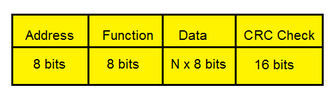
\includegraphics[width=.5\textwidth]{rtu_packet.png}
	\caption{Pacote da comunicação RTU}
	\label{fig:rtu_packet}
	%\source{Fornecido junto com os pontos}
\end{figure} 
\subsubsection{Modo de transmissão TCP}
O modo de transmissão TCP é uma aplicação do protocolo MODBUS baseado em TCP/IP, consequentemente utilizando a conexão ethernet. Para a pilha de comunicação, nesse protocolo é adicionado ao quadro um cabeçalho MBAP (MODBUS Application Protocol), deitando o modelo de mensagem como a figura \ref{fig:tcp_packet}:

\begin{figure}[h]
	\centering
	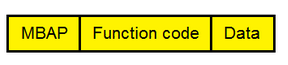
\includegraphics[width=.6\textwidth]{tcp_packet.png}
	\caption{Pacote da comunicação TCP}
	\label{fig:tcp_packet}
	%\source{Fornecido junto com os pontos}
\end{figure}
Esse novo cabeçalho tem 7 bytes de tamanho sendo composto por os seguintes elementos:
\begin{itemize}
	\item Transaction identifier: usado para identificação da resposta para a transação (2 bytes);
	\item Protocol identifier: 0 (zero) indica Modbus (2 bytes);
	\item Length: contagem de todos os próximos bytes (2 bytes);
	\item Unit identifier: utilizado para identificar o escravo remoto em uma rede Modbus RTU (1 byte).
	
\end{itemize}

O Modbus  TCP nao utiliza um byte de checkagem ao final da mensagem, pois o pŕoprio frame ethernet já apresenta uma checagem do tipo CRC-32. Na comunicação o cliente Modbus TCP inicia a conexão com o servidor para enviar as requisições, onde a porta padrão para a conexão com os servidores é a TCP 502.


\chapter{Estudos preliminares para a implantação de uma PCH}\label{cap:CnptDsng}
Os estudos preliminares representam todos os estudos que são feitos antes da implementação de uma PCH.
\section{Estudos Topográficos}
São feitas levantamentos topográficos da região, sendo elas: o estudo para determinação a queda natural do local, estudo das áreas de implantação das estruturas, local para empréstimo de solo, nivelamento a linha d'água do reservatório e cadastro jurídico das propriedades, todas de acordo com a norma a ABNT NBR 13133.
\section{Estudo de Inventário}
O estudo de inventário se dá pelo estudo de todo potencial do rio, afim de achar o lugar mais propício para instalação da  PCH. Não sendo considerado somente o potencial hidráulico mas também os possíveis impactos da construção.

\section{Estudos Geológicos e Geotécnicos}
Têm o objetivo de investigar as condições das fundações da obra, buscando também áreas para recursos de construção, jazidas de minerais e também determinando locais para instalações de obra como o canteiro.

\section{Estudos Ambientais}
Os impactos ambientais envolve toda parte dos efeitos da inundação e da construção a natureza, o primeiro passo é a realização de um relatório ambiental preliminar - RAP e deve ser entregue para o órgão ambiental responsável. 
O documento deve conter os seguintes tópicos: Justificativas do empreendimento, caracterização do empreendimento, com os dados da usina e reservatório, diagnóstico ambiental preliminar, com os principais aspectos físicos, bióticos e antrópicos a região já levantados, identificação preliminar dos impactos, prováveis medidas mitigadoras e programas ambientais.
No final, ao ser aprovado o RAP, obtém-se a Licença Prévia - LP que é a autorização para iniciar a construção da obra a usina.

\chapter{Escolha do local para implantação da PCH}
\section{Método de Seleção}
Além do estudo preliminar do rio, é necessário analisar 3 itens para saber a viabilidade a construção da PCH, são elas: recursos hídricos, queda d'água e linha de transmissão próxima. Não adianta possuir um rio com ótimo potencial hidrelétrico se não tiver uma linha de transmissão para transportar essa energia, que possui um grande custo de instalação.

\section{Rio Itanhém}
O rio escolhido foi o Rio Itanhém, que nasce na aldeia dos Machacalis no município de Fronteira dos Vales ,estado de Minas Gerais e corre de oeste para leste até a foz em Alcobaça na Bahia, onde deságua no Oceano Atlântico.Sua escolha se deu ao fato de que não possui até o momento nenhuma PCH instalada e possui vários municípios próximo como: Teixeira de Freitas, St. Antonio de Barcelona, Nova Lídice e São José de Alcobaça que poderão desfrutar e até mesmo ser alvo de investimento futuramente.
O rio possui grande potencial hidrelétrico possuindo em média uma vazão de $35m^3/s$ sem muita variação durante o dia. Na imagem \ref{fig:vazao} descreve a vazão durante o ano:
\begin{figure}[h]
	\centering
	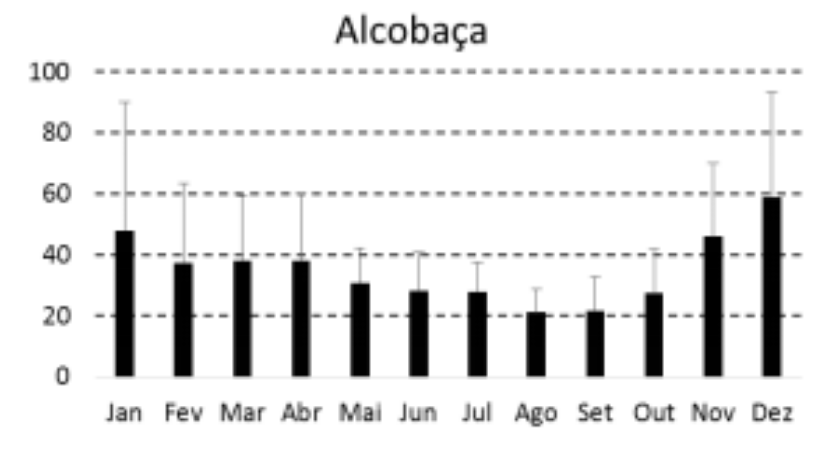
\includegraphics[width=.6\textwidth]{vazao.png}
	\caption{Distribuição a vazão ao ano do rio alcobaça}
	\label{fig:vazao}
	\source{[10]}
\end{figure}

\section{Área de Implantação da usina}
Foi percorrida toda a excursão do rio e o melhor lugar possui as seguintes características: um corredor estreito que facilita a construção da barreira, queda natural de 5m, área vizinha já degradada, poupando de desmatamento, área de empréstimo de solo contendo areia e cascalho e nenhuma população por perto. O local está indicado na imagem \ref{fig:geral}, onde o círculo vermelho ilustra a área de inundação, o círculo branco a área com construções e a linha vermelha indica o local da Barragem:
\begin{figure}[h]
	\centering
	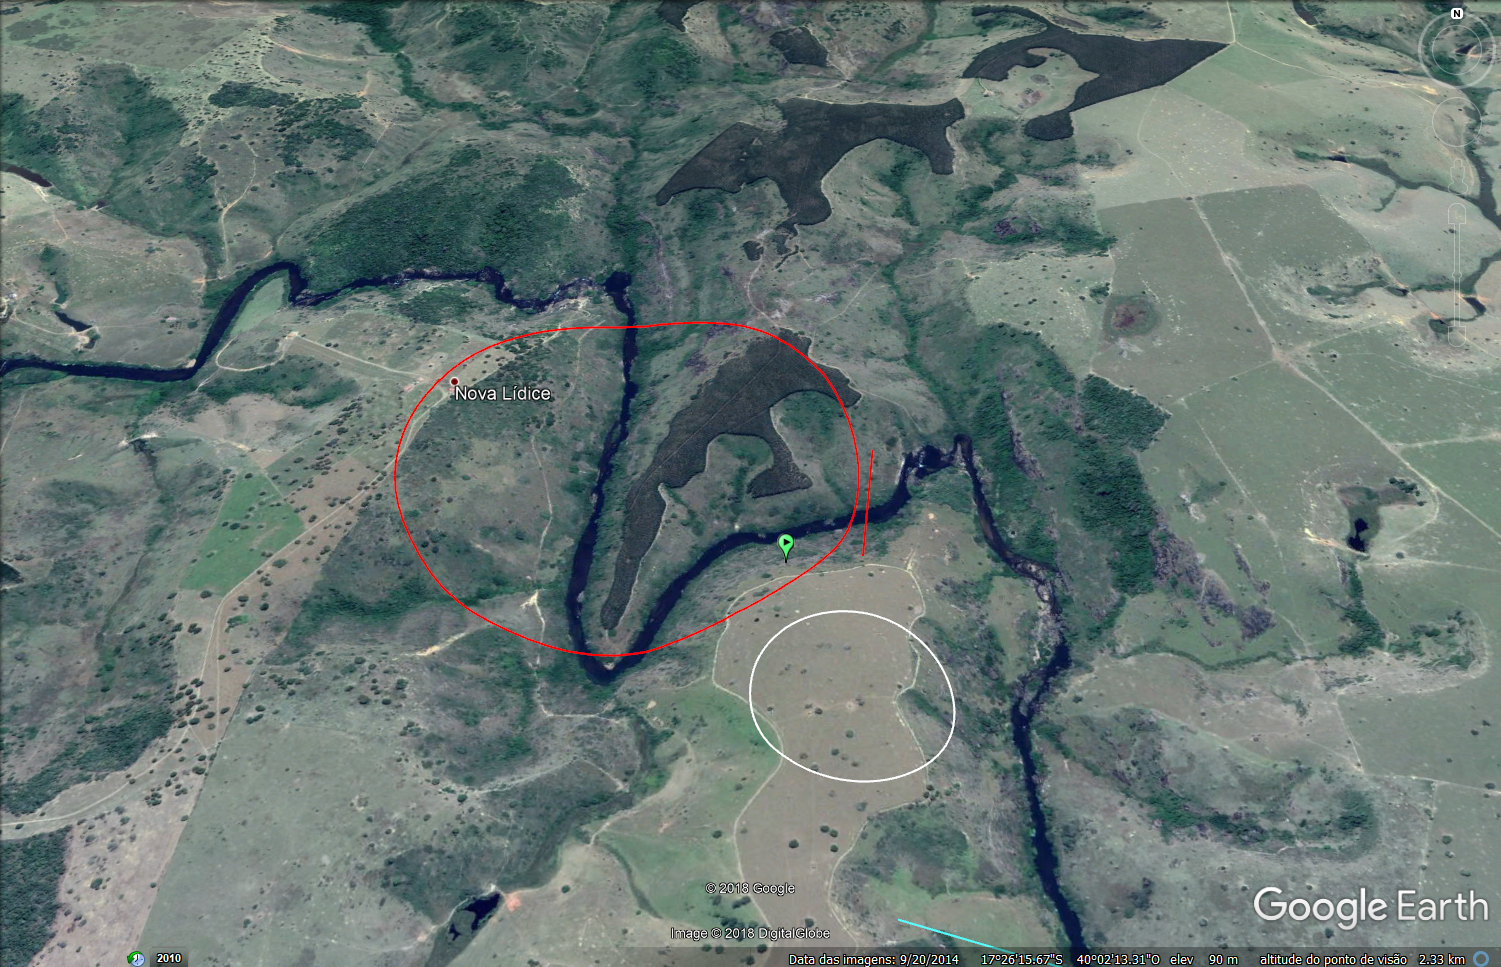
\includegraphics[width=.6\textwidth]{geral.png}
	\caption{Mapa da área escolhida}
	\label{fig:geral}
	\source{Google Earth Pro}
\end{figure}
O local para a barragem está mostrado na figura \ref{fig:alta2}, assim como o perfil de relevo.
\begin{figure}[h]
	\centering
	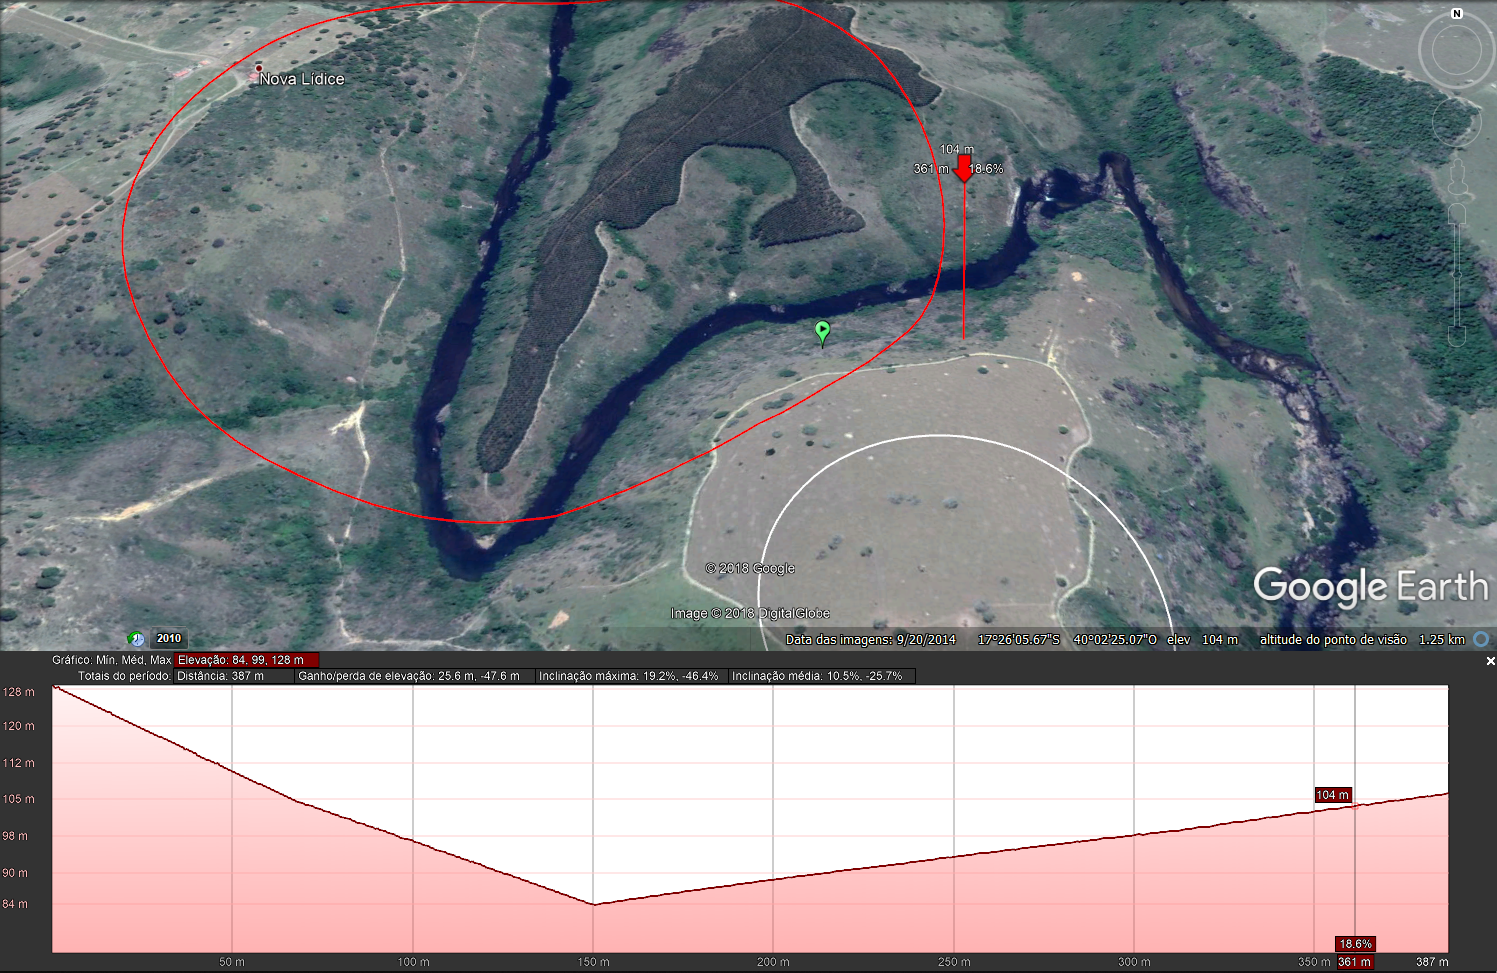
\includegraphics[width=.6\textwidth]{barreira_alta2.png}
	\caption{Mapa da área escolhida}
	\label{fig:alta2}
	\source{Google Earth Pro}
\end{figure}

\chapter{Especificações Técnicas}
As especificações técnicas levaram em consideração os valores reais disponíveis para projeto, quando não encontrados, foram estipulados valores baseados em pesquisas e projetos semelhantes.
\section{Barragem}
A barragem é uma estrutura que tem a função de represar a água em uma determinada altura. Essa altura e a taxa na qual a água flui do reservatório através das turbinas determina quantidade de eletricidade que pode ser gerada. Isso pode ser calculado usando a equação de energia hidrelétrica. À medida que a altura da barragem aumenta a quantidade de eletricidade gerada também aumenta. No caso de hidrelétricas situadas em locais com baixa queda, a barragem tem também a função de criar o desnível necessário à produção da energia desejada. Atualmente no Brasil tem se adotados os seguintes tipos de barragem: de terra, enrocamento e concreto.

Para o projeto foi escolhido uma barragem de terra, pois o local escolhido para construção da PCH apresenta uma topologia suave e vales pouco encaixados. Como o solo da região é tipicamente arenoso selecionamos uma seção trapezoidal conforme a imagem abaixo.
\begin{figure}[h]
	\centering
	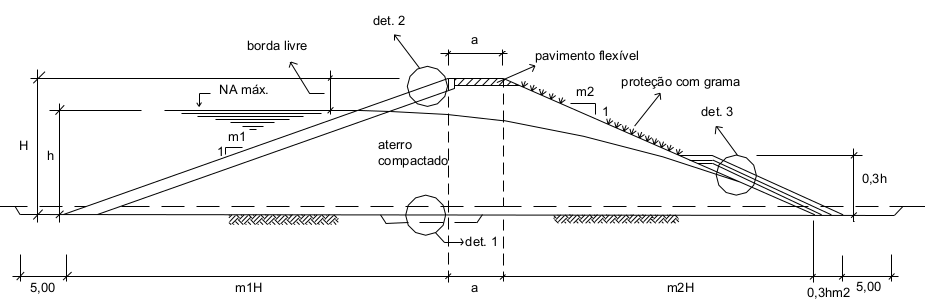
\includegraphics[width=1\textwidth]{barra_homo.png}
	\caption{Projeto de barragem Homogênea}
	\label{fig:barra_homo}
	\source{Manual da Eletrobrás}
\end{figure}

A largura da base da barragem é dimensionada conforme a equação de número 1. Onde a largura da crista ($a$) deverá ser de pelo menos 3 metros, a altura da barragem é dada por (H), a inclinação do talude de montante ($m_1$) e a inclinação de jusante ($m_2$) são definidas pela tabela 1.
\begin{equation}
	b = a + (m_1 + m_2)*H
\end{equation}

\begin{figure}[h]
	\centering
	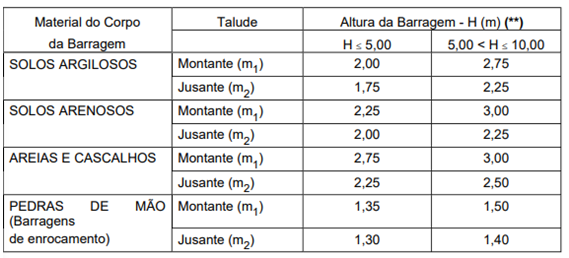
\includegraphics[width=.8\textwidth]{tab_solos.png}
	\caption{Tabela para projeto da barragem}
	\label{fig:tab_solos}
	\source{Manual da Eletrobrás}
\end{figure}
Aplicando o cálculo no nosso projeto definindo a altura da crista como 3 metros e a altura da barragem como 10 metros obtém-se o se valor de comprimento:
\begin{equation}
b = 55,5 m
\end{equation}

\section{Vertedouros}
Vertedouro é uma estrutura que permite o controle do nível da água de um reservatório, principalmente em períodos de cheias.  O vertedouro é uma das partes mais importante de uma usina hidrelétrica, pois se houver muita água passando pela barragem, elementos como as turbinas não podem funcionar adequadamente e podem ser danificados. Os vertedouros protegem essas outras partes de danos ou complicações.

Todo reservatório hidrelétrico tem certa capacidade ou quantidade de água que pode conter. Se o reservatório já estiver cheio, mas as águas da enchente entrarem no reservatório, o nível da água aumentará e isso poderá resultar na sobreposição da barragem. Os vertedouros são construídos para evitar isso, pois permitem que seja extraído um pouco de água do topo do reservatório para dar espaço à nova água. Quando um reservatório está cheio, seu nível de água será igual à altura do vertedouro. Assim que qualquer excesso de água entrar no reservatório, a água começará imediatamente a fluir através do vertedouro.

Para dimensionar a largura de um vertedouro em canal, com seção trapezoidal mostrado a figura \ref{fig:vertedouro}, deverá ser levada em conta a vazão máxima de projeto ($Q_{max}$), a inclinação dos taludes ($m$), a lâmina d’água máxima ($h_{max}$), a velocidade máxima admissível no canal ($V_{max}$).

\begin{figure}[h]
	\centering
	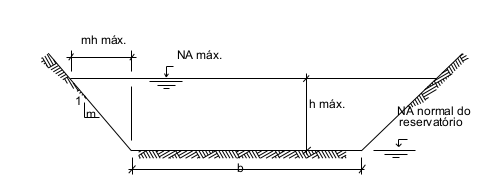
\includegraphics[width=.8\textwidth]{vertedouro.png}
	\caption{Desenho técnico do vertedouro}
	\label{fig:vertedouro}
	\source{Manual da Eletrobrás}
\end{figure}

\begin{equation}
b = \dfrac{Q_{max}-V_{max}mh^2_{max}}{V_{max}Q_{max}}
\end{equation}

Escolhendo um vertedouro com taludes de argila dura, temos um $m=0,75$, considerando a velocidade máxima de $1,7m/s$ e uma altura de $1m$. É obtido um valor de :
\begin{equation}
	b=19,83
\end{equation}

\section{Chaminé de Equilíbrio}
A chaminé de equilíbrio é uma espécie de reservatório com eixo vertical, normalmente posicionado no final da tubulação de adução de baixa pressão e a montante do conduto forçado.  Ele é usando para amortecer as variações de pressão que se propagam pelo conduto forçado e armazenar água para fornecer ao conduto forçado o fluxo inicial provocado pela nova abertura da turbina, até que se estabeleça o regime contínuo. Quando necessário, a chaminé de equilíbrio deve ser instalada o mais próximo possível da casa de força, para reduzir o comprimento do conduto forçado e diminuir os efeitos do golpe de aríete.

A verificação dessa necessidade é feito pelo cálculo do critério da constante de aceleração do escoamento no conduto forçado como mostrado abaixo.
\begin{equation}
t_h = \dfrac{V_{cf}L_{cf}}{gH_b}
\end{equation}
Onde $L_{cf}$ é o comprimento do conduto forçado,Hba queda bruta e $V_{cf}$ a velocidade de escoamento no conduto forçado. Para $t_h < 3$ não há a necessidade de instalação da chaminé. Entre $3$ e $6$ é desejável mas não obrigatória. Para $t_h> 6$  é obrigatória a instalação da chaminé.

A instalação de uma válvula de alívio na entrada, ou na caixa espiral da turbina, pode evitar a necessidade da chaminé. No entanto, essa solução deve ser analisada criteriosamente, considerando a segurança que deve haver na abertura da mesma, em caso de fechamento rápido do distribuidor.

\section{Conduto Forçado}
Conduto forçado é definido como uma tubulação de grande diâmetro, podendo ser composto de aço, concreto, fibra de vidro e PVC. São projetados para tolerar altas tensões por causa da pressão estática da coluna d’água e também por causa do golpe de aríete criado pelas mudanças bruscas no fluxo d’água, e pode ser realizado pelo fechamento e aberturas de válvulas e/ou distribuidor da turbina.

O conduto forçado pode ser projetado para ficar exposto ou enterrado. Se for exposto deve ser fundido em berços de concreto ou pedra. Vai depender da topografia da propriedade para delimitar o número de condutos, pode-se ter um conduto para cada máquina hidráulica ou ainda um com diâmetro maior que se ramifica em outros criando uma bifurcação de diâmetros menores de acordo com o número de máquinas.
O diâmetro da tubulação é definido através do cálculo de diâmetro econômico pela fórmula de Bondshu.
\begin{equation}
	D_e = 127\sqrt[7]{\dfrac{Q^3}{H_b}}
\end{equation}
Onde $H_b$ é a queda bruta, $Q$ a descarga máxima na tubulação e $D_e$ o diâmetro econômico. Depois de feito esse cálculo deve-se verificar se a velocidade máxima admissível de acordo com a fórmula abaixo e para cada material está conforme a tabela 3.
\begin{equation}
	V_{adm} = \dfrac{4Q}{nD^2_e}
\end{equation}

\begin{figure}[h]
	\centering
	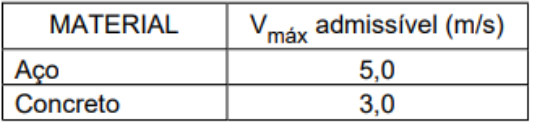
\includegraphics[width=.6\textwidth]{tab_conduto.png}
	\caption{Desenho técnico do vertedouro}
	\label{fig:tab_conduto}
	\source{Manual da Eletrobrás}
\end{figure}

Adotando um Conduto forçado de concreto com uma descarga máxima de $1 m^3/s$ e uma queda bruta de $15m$. Obtém um valor de $D_{e}=84,01$ cm e $V=1,8$ m/s, a velocidade encontrada é aceitável, pois ela é inferior à máxima permitida.

\section{Tomada D'agua} 
A tomada d’água é responsável pela captação de água para fazer a turbinar gerar energia. A estrutura de tomada d’água deve ser localizada, sempre que possível, junto à margem do reservatório, ao longo de trechos retos. Nos trechos em curva, a tomada d’água deve ser posicionada do lado côncavo, pois os sedimentos transportados pelo escoamento, na maior parte, se depositam na parte convexa. Ela é composta por três componentes essenciais: grade de proteção, comporta e tubo de aeração.
A função da grade de proteção é evitar a entrada de detritos, folhas e lixo para evitar danos nas turbinas. Normalmente, ela é uma tela composta por várias barras de aço paralelas, preferencialmente na vertical, localizada na entrada da tomada de água.

\section{Casa de força}
A casa de força é o lugar onde se encontra as turbinas e os geradores. É essencial a existência de uma sala de controle dentro da casa de força, pois é onde os engenheiros podem regular as válvulas controlando o fluxo de água nas turbinas ou monitorar o desempenho de cada unidade até a rede elétrica principal. É calculada a sua dimensão baseada no tamanho necessário para armazenar todos os itens do seu inventário, essa perspectiva não foi abordada no projeto.

\section{Subestação}
A subestação será do tipo Conjunto de manobra e controle blindado, conforme definido pela norma ABNT NBR 6979, esse tipo de subestação proporciona melhores condições de segurança pessoal contra riscos de acidentes e maior rapidez na fase de instalação do equipamento na usina.

Devido que a PCH trabalhará em sistema isolado, a utilização de relés de sobrecorrente com características de tempo inverso associados a relés de sobrecorrente instantâneos é uma solução economicamente interessante.

Os elementos utilizados seguiram a suas respectivas normas no seu projetos, podemos citar: disjuntores, com a norma NBR 7118, Seccionadores, com a norma NBR 6935,para-raios, a norma NBR 5287 e IEC 99-4, transformadores de potencial indutivo, a norma NBR 6856, transformador de corrente , a norma NBR 6855, assim garantindo um sistema com alta confiabilidade.

\section{Turbina}
Para atender as especificações do projeto, foi escolhida a turbina francis, devido a sua faixa de operação boa para baixas quedas. “No âmbito destas Diretrizes, a turbina Francis atende a quedas de 15 a 250 m e potências de 500 a 15000 kW possuindo ótimas características de desempenho sob cargas parciais de  até 70\% da carga nominal, funcionando ainda adequadamente entre 70 e 50\% da carga, embora com perda progressiva do rendimento. Não é aconselhável o funcionamento da turbina“(ELETROBRÁS,2000).

Foram feitos os cálculos relativos à turbina, considerando uma potência desejada de 4500MW, sendo maior que a energia firme, assim sendo calculado uma velocidade de rotação de 181,79 rad/s, por meio da fórmula:

\begin{equation}
	n_{rot}= \dfrac{K*H^{0,75}_{liq}}{P_{turb}^{0,5}}
	\end{equation}

O diâmetro de saída da turbina é calculado utilizando a rotação da turbina $n$ e um coeficiente de velocidade $k_u$ obtido por meio da $rotação específica$ e a altura da queda líquida, por meio do seguinte cálculo:
\begin{equation}
	D_{saída}=(84,5k_uH^{0,5})
\end{equation}
Sendo encontrado um diâmetro de saída da turbina de $D_{saída}=16,93$, utilizando a queda conhecida de $H=15m$, outros parâmetros cálculados que também são importantes de se destacar são, a velocidade específica $n_s$, com um valor de $3383,588$.

\section{Geradores}
\subsection{Potência nominal}
A potência nominal do gerador deve ser maior que a da turbina, a mesma foi calculada levando em consideração um fator de potência de 0,8 e um rendimento de 97\%, de acordo com a seguinte fórmula:
\begin{equation}
P_{gerador} = \dfrac{P_{turbina}*n_{gerador}}{fp}
\end{equation}
Sendo encontrado um valor de potência para o gerador de $P_{gerador} = 5456,25$.

\subsection{Tensão de Geração}
A escolha da tensão de geração deve considerar não só os custos do gerador, mas também os custos da interligação gerador–transformador e dos equipamentos ligados à tensão de geração. É desejável maior tensão de geração para diminuir as perdas de transmissão, contudo. de acordo com o manual de Diretrizes, a tensão economicamente atraente está relacionada com a potência do gerador, como mostra tabela a seguir:
\begin{figure}[h]
	\centering
	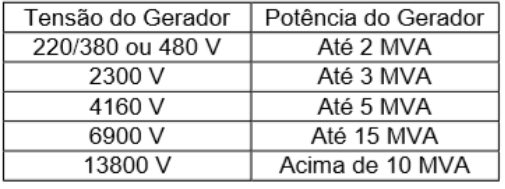
\includegraphics[width=.6\textwidth]{tab_ger.png}
	\caption{Tabela de tensão de geração econômicamente viável}
	\label{fig:tab_ger}
	\source{Manual da Eletrobrás}
\end{figure}
Como a potência encontrada foi maior que 5MVA a tensão do gerador será 6900V.
\subsection{Multiplicador de Velocidade}
A velocidade de rotação da turbina está relacionada diretamente com o número de polos do gerador, a figura \ref{fig:sincrona} mostra essa relação. Como a velocidade de rotação encontrada foi muito baixa, será utilizado um multiplicador de velocidade na saída do gerador. Esse multiplicador de velocidade tem geralmente 4,6 ou 8 polos, foi escolhido um multiplicador de 8 polos pois a velocidade é muito baixa.
\begin{figure}[h]
	\centering
	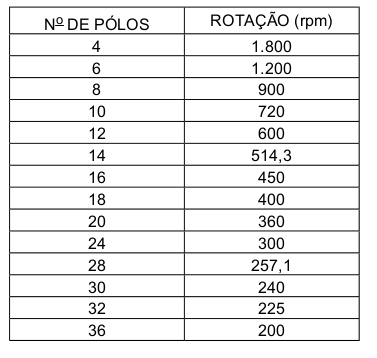
\includegraphics[width=.6\textwidth]{sincrona.png}
	\caption{Relação de número de Polos para velocidade de Rotação}
	\label{fig:sincrona}
	\source{Manual da Eletrobrás}
\end{figure}

\section{Transformador Elevador}
Na casa de força será utilizado um transformador que eleva a tensão do gerador de 6900V para 13800V, para posteriormente essa energia passar por outro transformador elevador, que eleva a tensão de $13,8KV$ para $138KV$ pois esse é o valor utilizado para a transmissão na regiao.

\section{Energia Firme e Potência Gerada ao ano}
A energia firme se dá pela energia bruta gerada pela PCH, dependendo dos valores de altura de queda $H_queda$, vazão média $Q_méd$ e gravidade. No caso do rio alcobaça a vazão média de $35 m^3/s$ e queda livre de 15 metros, resultando em uma energia firme de:
\begin{equation}
	EF = 5150,25 KW
\end{equation}

Para o cálculo da potência gerada ao ano, se levou em consideração a energia firme disponível, multiplicada pelo rendimento do conjunto turbina-gerador, e foi considerado um rendimento mecânico, referente às perdas nos túneis, vertedouro e canal.Foi considerado um rendimento mecânico fictício de 70\% e rendimento do conjunto turbina-gerador de 90\%.
\begin{equation}
P = g *(H*. Q_{méd} * n_{gerador} *n_{mecânico})
\end{equation}
Sendo assim encontrado um valor de potência gerada de $3,174MW$, representando uma energia anual de $27483,624 KWh/Ano$

\section{Linha de Transmissão}
É conhecido que o município de Teixeira de Freitas recebe a energia em $138kV$ da usina de Teixeira de Freitas 2, então, será estabelecida uma linha também de $138kV$ diretamene para a cidade. Foi encontrada um tamanho de linha de $31,79km$, partindo dp local de instalação da PCH para a cidade de Teixeira de Freitas. O caminho está mostrado na imagem \ref{fig:dist}
\begin{figure}[h]
	\centering
	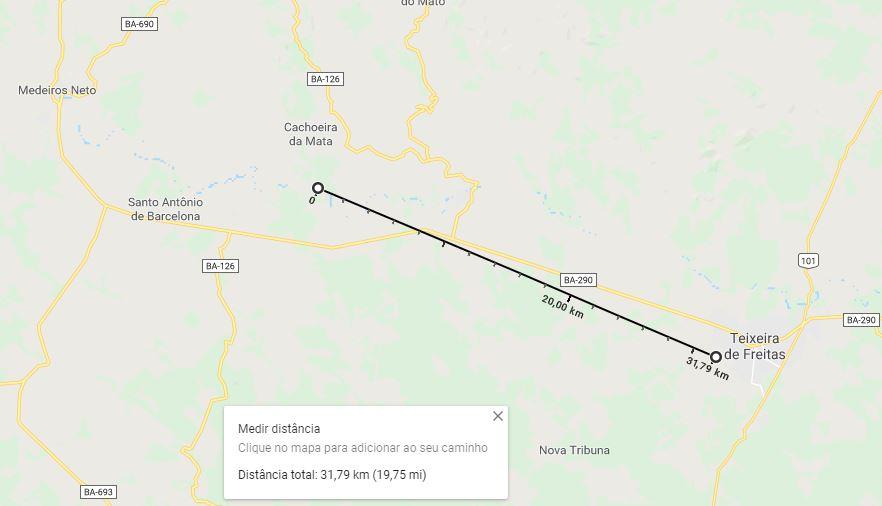
\includegraphics[width=1\textwidth]{dist_linha.JPG}
	\caption{Distância de linha entre PCH e Teixeira de Freitas}
	\label{fig:dist}
	\source{Google Maps}
\end{figure}

\chapter{Estudo da viabilidade financeira}
O estudo de custo foi feito de acordo com o custo de uma usina similar que será construída, sendo que os valores poderão mudar de acordo com a época do ano de construção. O valor total a usina foi de 98376740 reais, com o valor do MWh de 211 reais em aproximadamente 13 anos a PCH se pagará.
\begin{figure}[h]
	\centering
	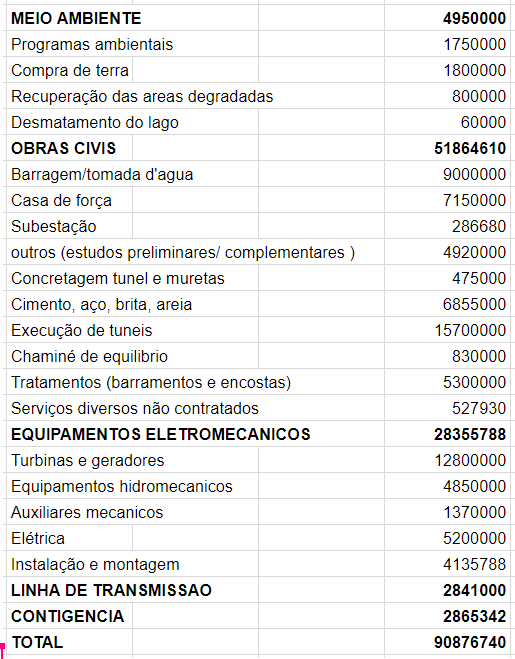
\includegraphics[width=.6\textwidth]{custom.png}
	\caption{Tabela de custos}
	\label{fig:custo}
	%\source{Manual da Eletrobrás}
\end{figure}

\chapter{Cronograma}
O cronograma deve contemplar todas as etapas para a implantação de uma PCH. Foi tomado como base de tempo um projeto semelhante mas, vale ressaltar que a obra pode sofrer atrasos durante a sua implantação, devido a fatores externos. O cronograma relativo da obra está mostrado no Anexo A.

\chapter{Conclusão}
O projeto de uma PCH nessa região se mostrou muito viável, o rio apresenta uma vazão interessante e o relevo encontrado também é propício para instalação de uma barragem. A vegetação reduzida e área já desmatada conseguem diminuir o impacto ambiental, e a localização também possibilita futuras implementações.

Entre as futuras implementações, é importante destacar a possibilidade de fornecimento paras os municípios de Medeiros Neto, e Teixeira de Freitas simultâneamente, além da localização da localização próxima da Usina de Santa Maria, que representa uma usina de geração de energia elétrica por meio de biomassa.

Para maximizar a fidelidade da análise de viabilidade, seria interessante realizar o trabalho em conjunto com engenheiros civis e mecânicos. Para encontrar a produção exata da turbina é necessário ter conhecimento de todas as perdas, sendo elas nas partes mecânica da usina, como é o caso dos dutos, tubos e construções , nas partes elétricas, como transformadores, turbinas e fios.

O projeto de PCHs se mostra uma importante prática, considerando que o brasil tem diversos rios, afluentes e a mesma possibilita diversos benefícios e um destaque importante é o desenvolvimento da área, a construção de usinas movimenta pessoas e dinheiro naquela região, estimulando também o crescimento.

Se conclui então que é viável a implantação de uma PCH nessa área, não levando em consideração somente os custos, por mais que os mesmos apresentem valores lucrativos, mas também pela facilidade da construção, possibilidade de fornecimento para municípios próximos e o estímulo para desenvolvimento da localidade.


%\chapter{Resultados}\label{cap:conclusao}
\section{Fluxograma do funcionamento}
\section{Prototipo}
\section{Funcionamento}
foto do programa funcionando
\lipsum[5]
\section{Conclusão}

\lipsum[5] 

% ----------------------------------------------------------
% ELEMENTOS PÓS-TEXTUAIS (Referências, Glossário, Apêndices)
% ----------------------------------------------------------
\postextual

   \markboth{}{}
\begin{center}
	\Large \textbf{Referências}
\end{center}
	
[1] ELETROBRÁS. Diretrizes para estudos e projetos de Pequenas Centrais Hidrelétricas. Eletrobras, 2000.

[2] WISSMANN, Leandro; GRANDO, Maurício Nelson. Estudo prévio da instalação de uma pequena central hidrelétrica no manancial do rio Pato Branco no estado do Paraná. 2012. Trabalho de Conclusão de Curso. Universidade Tecnológica Federal do Paraná - Disponível em: \url{http://repositorio.roca.utfpr.edu.br/jspui/handle/1/442}

[3] ABREU, Thiago Modesto de. Proposta de Metodologia para definição de quantidade de grupos geradores de pequenas centrais hidrelétricas. 2015. Disponivel em: \url{http://www.aneel.gov.br/documents/656835/14876412/Disserta%C3%A7%C3%A3o+Thiago+Abreu+2015.pdf/7d05c97f-4e45-054c-33c6-020884240fef}

[4] Mapa de linhas de transmissão e subestações - Sistema Interligado Nacional - Rede de Operação. Disponível em:  \url{http://sindat.ons.org.br/SINDAT/Home/ControleSistema}

[5] Características e requisitos técnicos básicos das instalações de transmissão - Subestação Teixeira de Freitas 2. Disponível em: \url{http://www2.aneel.gov.br/aplicacoes/editais_transmissao/documentos/Lote_L_Anexo_T%C3%A9cnico_Eun%C3%A1polis_Teixeira_de_Freitas_II_C2.pdf}
	
[6] ANEEL, ANDEE. Atlas de energia elétrica do Brasil. Brasília, 2008.

[7] BRONZATTI, Fabricio Luiz; IAROZINSKI NETO, Alfredo. Matrizes energéticas no Brasil: cenário 2010-2030. Encontro Nacional de Engenharia de Produção, v. 28, p. 13-16, 2008.

[8] Revitalização da câmara de carga e do conduto forçado da usina hidrelétrica de rio branco do sul.Disponível em: \url{<http://repositorio.roca.utfpr.edu.br/jspui/bitstream/1/6766/1/CT_COELE_2015_1_14.pdf>}

[9] Energy Education. Disponível em: \url{<https://energyeducation.ca/encyclopedia/Spillway>}

[10] CUSSIOLI, Mariana Coppede. Dinâmica da desembocadura do rio Itanhém, Alcobaça, BA. 2010. Tese de Doutorado. Universidade de São Paulo - Disponível em: \url{<http://www.teses.usp.br/teses/disponiveis/21/21133/tde-14092012-133655/en.php>}

\newpage
\thispagestyle{empty}
\hfill
\vfill
\begin{center}
	\textbf{{\LARGE ANEXO}}
\end{center}

\vfill
\hfill

\newpage
\thispagestyle{empty}
\begin{landscape}
	\begin{figure}[h]
		\centering
		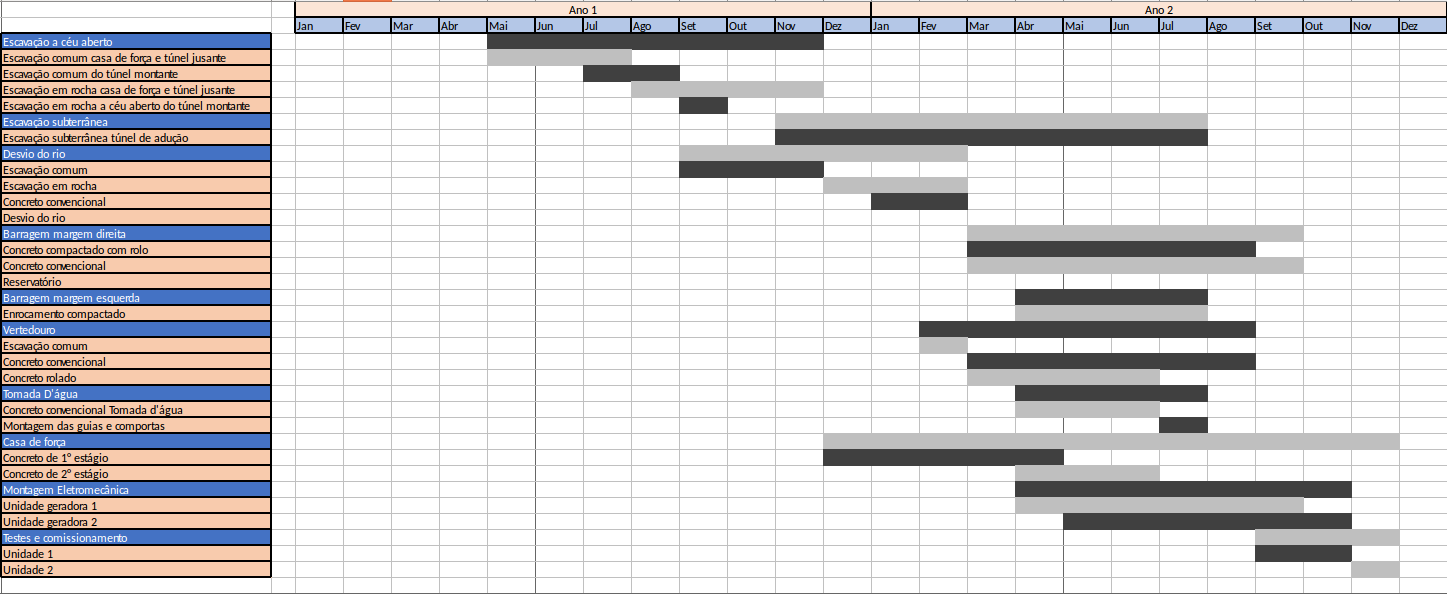
\includegraphics[width=1.6\textwidth]{cronos.png}
		\caption{Cronograma}
		\label{fig:cronos}
		\source{Cronograma do Projeto}
	\end{figure}
\end{landscape}

% Referências bibliográficas
%\bibliography{bibliografia}

%\printglossaries




% Índice remissivo (Consultar manual)
%\phantompart
%\printindex



\end{document}
